\documentclass[11pt,a4paper]{article}
\usepackage[utf8]{inputenc}
\usepackage{amsmath}
\usepackage{amsfonts}
\usepackage{amssymb}
\usepackage{graphicx}
\newcommand{\qed}{\hfill $\blacksquare$}
\author{Jake Bruner}
\title{Proof without words - Exploration}
\begin{document}
\maketitle
\tableofcontents
\pagebreak

\section{Introduction and Aim}

if there were one thing i wish my teachers emphasized more, would be the importance of the commutivity, associativity, identity and inverse properties. I vividly recall 7th grade me rollling my eyes in Ms. Lee’s Algebra class when we had to memorize the names. It felt all too much like mathematicians naming things to give the subject more importance. And as I’ve grown to appreciate the value of using well-defined terminology, I still believe it limits the accessibility of math’s fascinating applications and beautiful conclusions. 

group law on a torus; fractional linear transformations 
explain how this relates to the embedding of a elliptic curve in the complex projective plane
discuss how fractional linear transformations under SL(2,Z) give way to modular forms? 
how can the jacobian make abelian variety over any variety?

cycle graphs of elliptic curves

- start out with group theory first principals with some history and examples
- begin discussing how this structre arose everywhere in math, creating new fields of study
- talk about algebraic curves and how they were discovered to have group symmetry 
- begin with comic sections and their cyclic groups
- motivate elliptic curves as isomorphic to a direct product of groups 


exponentiation is defined over any associative algebra?!

So I want to pose a question. For some the answer might be obvious, but I know that I was amazed by the answer when I first learnt about it. If I want to communicate with someone and I haven’t established a password or cipher or secret language, can you think of a feasible way to establish a secure line of communication (for instance a using secret password, or text scrambling) over an eavesdropped channel such that the eavesdropper cannot work out the common secret? 

At first glance, some people—or at least myself—would be inclined to retort the impossibility of such a mechanism. Since logically, if you haven’t established an encryption scheme with some shared secret ‘unlocker’ (which we will define as symmetric cryptography) it seems impossible to do so over an eavesdropped channel 

…

If you’re particularly clever (i argue ingenious) you might recall back to grade school when we get intuition for the fact that multiplying numbers together is generally easier to do than dividing. So hypothetically, if two communicators both shared a public number and then shared their number*the other’s public number, the result of the the number shared with their private number, each individual obtains the same result, except crucially an evesdropper can not. 

it’s important to sit for a moment and think about how powerful this is. that you can talk to any unknown party that you have never spoken to at all previously in such a way that an eavesdropper of the entire extent of both parties communication cannot obtain the same secret. Even if this scheme or plan wasn’t prior established, one party could easily explain how the other party could follow it, since an eavesdropped knowing the scheme has no effect on its security (which is in stark contrast to how knowing the password to symmetric encryption renders it useless)

much akin to mixing paints in a bucket


*if instead of requiring a pre determined shared message, a common message is the only requirement. which for things like a common password is exactly perfect. 


\iffalse
\pagebreak
\section{Understanding Proof Through Pythagoras}
\subsection{The First Proof \textit{circa} 200 BCE}
\begin{figure}[h]
\begin{center}
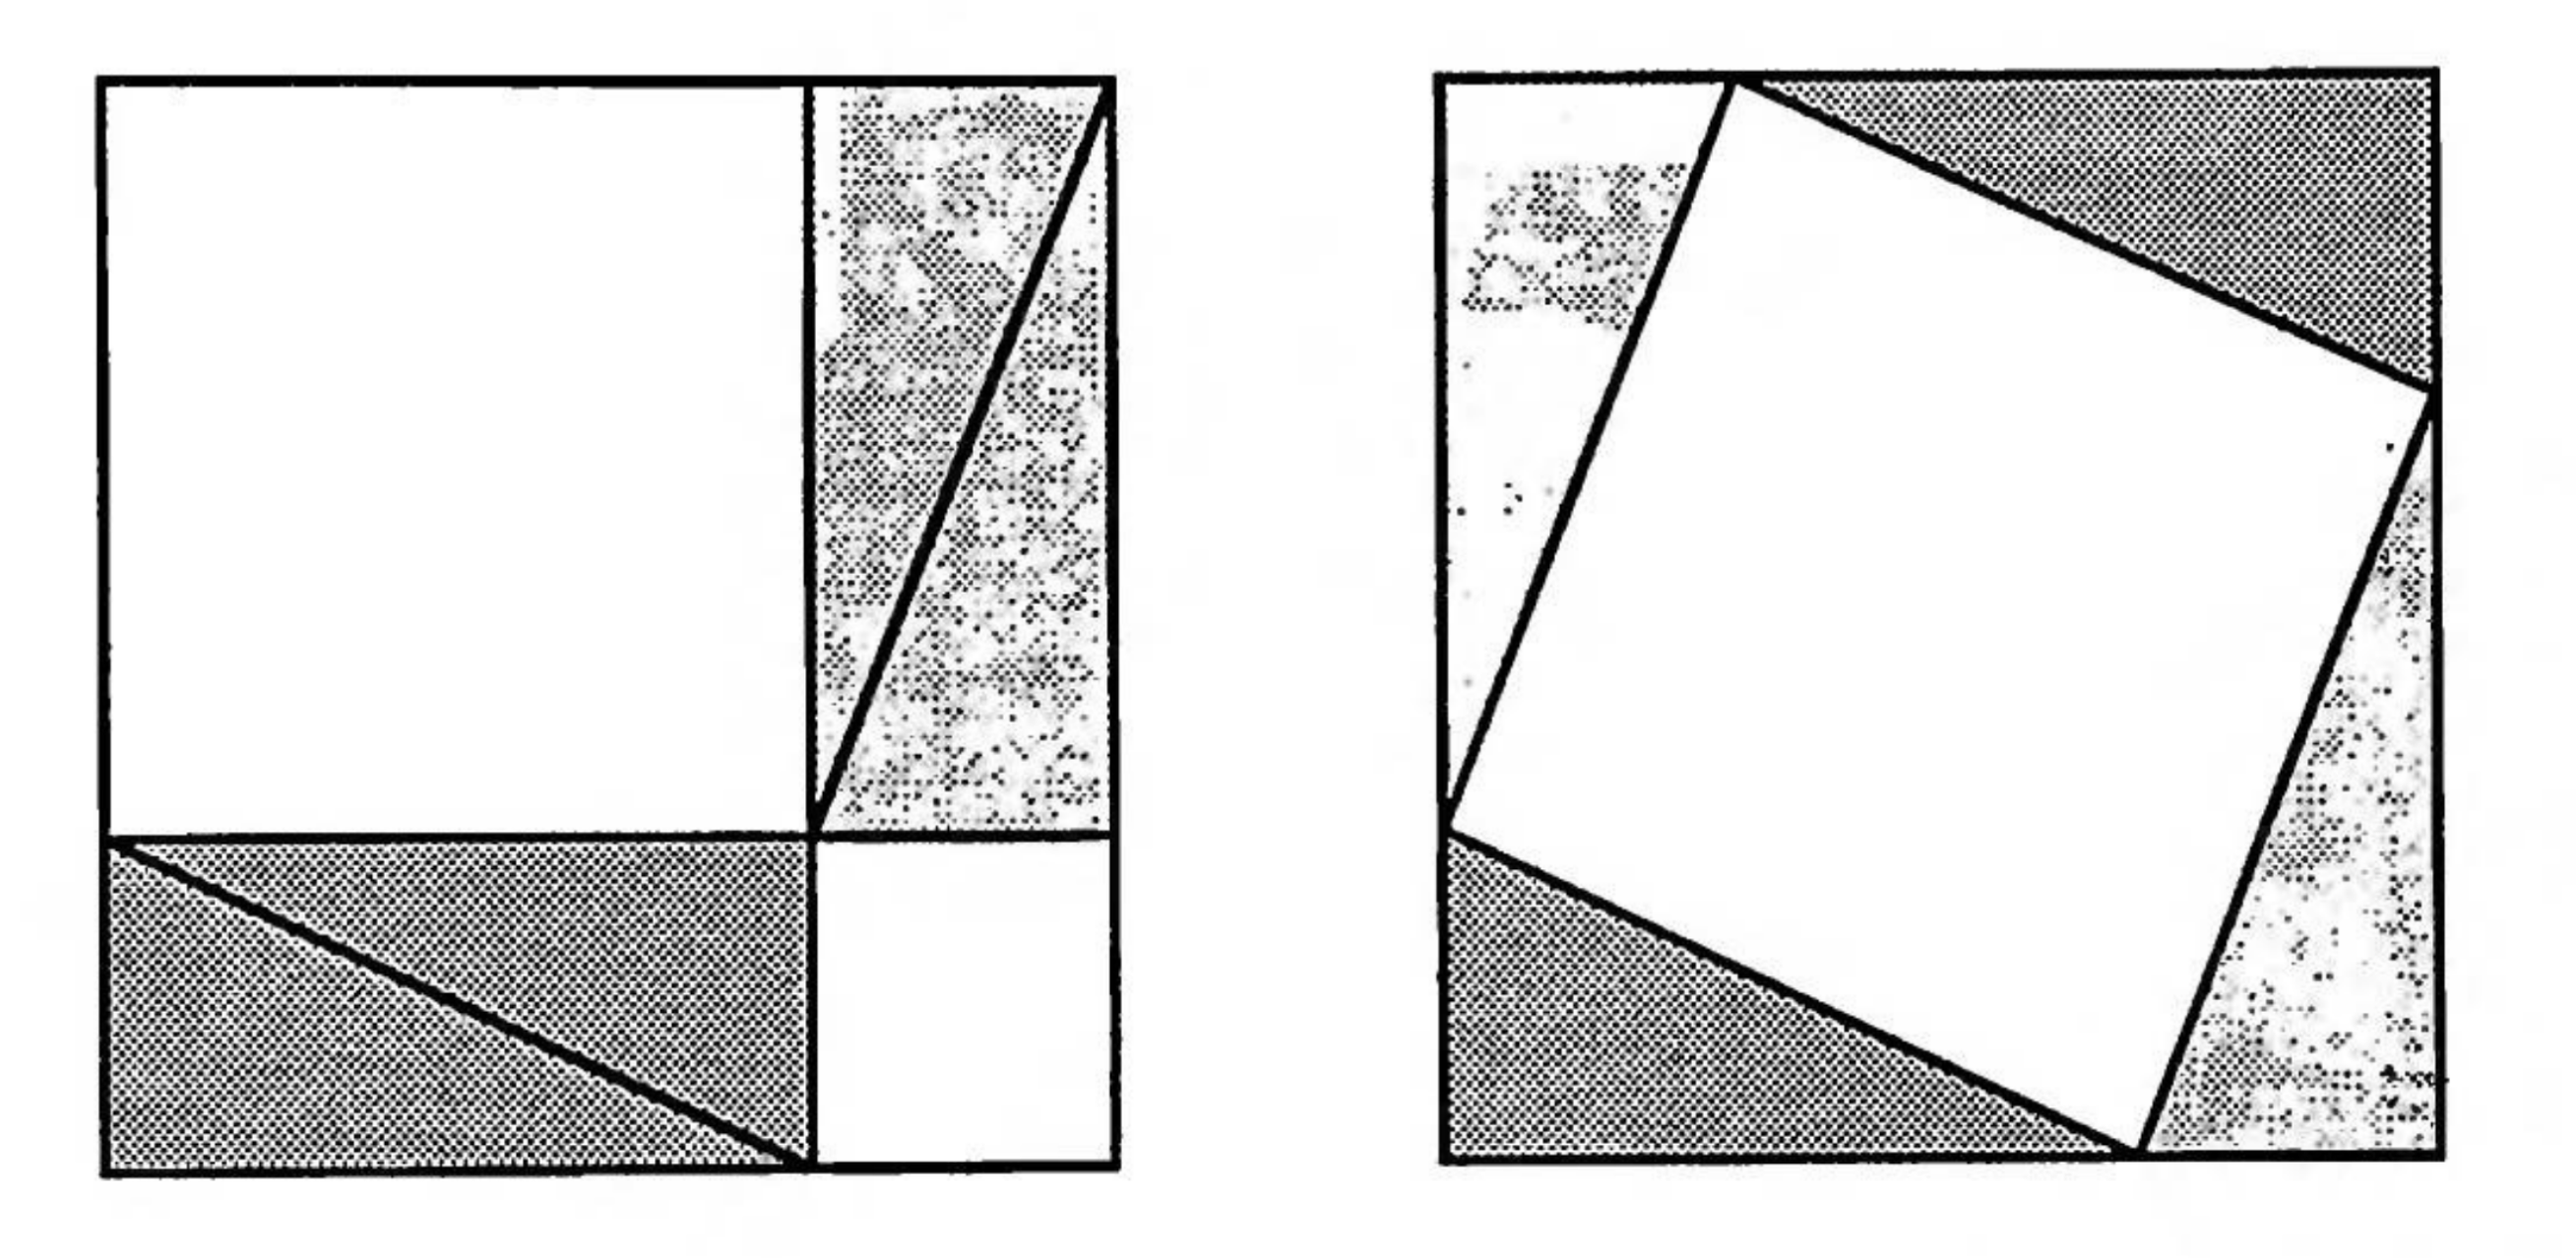
\includegraphics[scale=.20]{proof of pt} 
\caption{Proof of Pythagorean Theorem circa \textit{200 BC}}
\end{center}
\end{figure}
\fi

Take this visual depiction of the Pythagorean Theorem. The visual is using the properties of triangles and squares to show that all right triangles side's, $a$, $b$ are related to the hypotenuse $c$ by $a^2 +b^2 = c^2$.



With the diagram more clearly labeled, its obvious that the four congruent right triangles are transformed into two orientations, where in the first orientation, the two white spaces are equivalent to $a^2$ and $b^2$ respectively, and in the second, the white space is equivalent to $c^2$. And although it holds true for this specific triangle, it's not initially obvious how this construction behaves for other right triangles. Explained more thoughtfully, assume that a right triangle is flipped across one of its non-hypotenuse axis and joined with the first to create a rectangle. If another congruent rectangle is rotated perpendicular, and the two rectangles are placed such that they form two squares, then the squares will have area equal to the square of side one and side two respectively. Now consider shifting the four triangles such that the hypotenuses enclose a closed square with area equal to the square of the hypotenuse. Since the total area enclosed by the construction was kept constant and the four triangles remained congruent, it follows that the areas $a^2 +b^2$ is equivalent to $c^2$.
\pagebreak
\subsection{Comparison to Alternative Methods}

Taking this more traditional algebraic proof of Pythagoras' Theorem, its clear there are many differences in presentation. Most obviously, this proof uses an extensive amount of equations and text to describe its construction and assumption. By contrast, the visual proof simply relies on the reader's prior understanding of shapes and forgoes any text or variables for its construction. Another key difference is the apparent rigor of the proof, since the contradictory proof's use of variables and equations conveys that this process would work for any side lengthed right triangle. This contradictory proof also states explicitly where it makes its assumption and where that assumption leads to a contradiction. Whereas, the visual proof doesn't use contradiction and doesn't state explicitly what element of the diagram proves the theorem.\\ \\
More broadly, the proofs we have explored within math class are much more oriented towards rigour, as opposed to visualisation or geometry. One downside of this approach is that our proofs, albeit correct, often don't answer "why" a theorem works. For instance, our proofs of irrationality for a number expressed as a logarithm or irreducible root feel quite hand-wavey and incomplete. The general process is to assume it is rational and can be expressed as a reduced fraction of integers, then demonstrate that the numerator and denominator share a common factor, hence the supposition is false. Proving anything in this matter doesn't provide a tangible feel for "why" something's true, but rather reaffirms the fact that it is true. Because of this short-coming, visual proof can often provide an extent of insight and understanding much greater than that of proof by contradiction or proofs relying on obscure properties or theorems.

\subsection{Are Proofs-Without-Words Proofs?}
According to Nelson in \textit{Proofs Without Words}, "of course, 'proofs without words' are not really proofs" (vi). I believe that in the most bland, uninspired, and pedantic way, this statement is true. However, given any room for creativity and perspective, I strongly believe that some proofs without words are absolutely proofs. In many ways, visualizations are an amazing tool at making an obscure mathematical fact accessible to a wider audience, since they often highlight key insight in a rigorous way without being too proof-like. Often math comes across as needlessly complicated, which I believe is a byproduct of an obsessive drive to abstract and generalise. People become extremely caught-up in describing the generalized theorem prior to teaching or learning an example or case of a law. For many people, this makes Mathematics as a subject incredibly opaque. \\ \\
	Take, for example, learning vectors. If an individual were to begin by learning that a vector space over a field $F$ is a set $V$ such that, the Cartesian product of two elements $V \times V$ maps to another element of $V$ and that a scalar $F \times V$ maps to another element $V$ etc etc, the individual will be able to apply nothing but recite a formal definition. Whereas, learning that a vector is an point with a direction and magnitude in physics, or a one-dimensional array in computer science, provides a much more useful understanding of how one would go about using vectors and why they might be useful. Similarly to proofs without words, learning these specific examples may not provide a rigorous and general explanation of a vector space, but they all prove helpful in aiding in assimilating opaque topics. Hence, I strongly disagree that proofs without words are not proofs, because in many ways, they provide more insight into a property or theorem than, for example, a rigorous proof by contradiction would.

\subsection{Exemplifying the Beauty of Wordless Proof}
Consider Figure 4, a visual proof from page 5 of \textit{Proofs Without Words}. \\

I believe this proof beautifully illustrates that the squares of the side lengths occupy an area equivalent to the square of the hypotenuse. Often, the idea of squaring a number is an abstract manipulation of a value, so by representing this as area, the visual is able to more meaningfully convey how these values relate to one and another. The proof supposes that the shaded area, constructed to equal the sum of the squares of the two sides, can be area-preservingly manipulated to fill the lower square. Now despite satisfying the intuition of the theorem, this proof fails to thoughtfully demonstrate how each step is preformed mathematically. For instance, the second and third panel both leverage the idea of closing the area from both sides into a neat shape with parallel lines extended from the lower square and a right angle from the perpendicular lines extended at the top. I almost imagine this as pushing together a constant volume of liquid from both sides into a neat shape. The not-so-obvious mathematical insight is that the triangle constructed by slicing the square with a line through a vertex can be transformed into the imagined rectangle above. Then the diagrams follow by showing that this newly formed shape, when dropped into the square, occupies the area equal to the hypotenuse squared. \\ \\
Although I appreciate this diagram visually, I think it lacks in its ability to convey the mathematical steps necessary to describe this diagram with rigour. As outlined previously, this highlights the nature of proof without words in general, because like most, this proof provides the "why"--notably that the area constructed from squares of the legs of a right triangle fits exactly into the area enclosed by the square of the hypotenuse--yet isnt 100\% clear in what steps it took. Again, I believe a proof like this provides more insight into the pythagorean theorem than the proof by contradiction did because it leverages the real-world concept of area or volume as opposed to the abstract concepts of algebra and exponents.

\pagebreak
\section{When Visual Proof Becomes Hectic}

Consider Richard Courant's proof of integration by parts: 



This proof--although rigorous--is an extremely confusing jumble of variables upon first glance.  Without text to aid, a few key assumptions are not immediately obvious. For instance, Courant's proof includes that the curve is bound by the parametric equation, $ \big( f(x), \ g(x) \big) $, made worse by the fact $x$ is the parameterising variable.  Furthermore, this 'visual' proof either requires the reader to figure out or have prior knowledge of how to integrate a parametric curve. Overall, the beauty of this proof cannot be realised without close examination, which detracts from its accessibility.
\pagebreak

Attempting to depict this proof in a more straight-forward way, it might be useful to relabel the axis and variables to be more friendly to math conventions. \\

Breaking this down piece by piece, it's initially helpful to reiterate these parametric equations in terms of non-parametric functions so that integration and derivation are more explicit. Parametric curves are easier to digest conceptually when they are discussed in reference to the path a vector draws. In this example, it is possible to imagine a 2d vector with $x$ component $f(t)$ and $y$ component $g(t)$.  As the variable $t$ sweeps through inputs (for example, time increasing from zero continuously) the output/head of the vector will draw out a continuous curve. So clearly here,  $y$ is a function of $x$ (even if its not explicitly--or technically implicitly--defined since $y$ varies according to whatever value $x$ takes on) and vice-versa.
\begin{align*}
x(y) &= x = f(t)\\
y(x) &= y = g(t)
\end{align*}
Given that these variables simply correspond to the x and y axis, it is possible to understand these integrals without knowing the process for parametric curves. Simply put, if one knows that an area under a curve can be represented by an integral with respect to the axis variable (usually $x$), it should logically be a similar process to see the area bounded by the vertical axis.  For the x axis, the area in the blue is simply:
\begin{align*}
A_b = \int_{x_1}^{x_2} y\ dx
\end{align*}
Now, the area bound by the curve and the y-axis takes the same form.  Although, for many this seems like sacrilege, this idea is perfectly legal; one can imagine this as defining the horizontal axis as $y$ and the vertical axis as $x$ then finding the area under a curve.  So hence, the area in red is simply:
\begin{align*}
A_r = \int_{y_1}^{y_2} x \ dy
\end{align*}
Now, the sum of these two integrals would represent the total area of the rectangular section of the graph,  minus the area in the white. Again,  the total area $A_b + A_r$ is equal to the large rectangle $x_2 \times y_2$ minus the small, white rectangle $x_1 \times y_1$.
\begin{align*}
A_b &+ &A_r &= &large\ rectangle\ &- &small\ rectangle \\
\int_{x_1}^{x_2} y \ dx &+ &\int_{y_1}^{y_2} x \ dy &= &( x_2 \times y_2)\ \ & - &(x_1 \times y_1)
\end{align*}
From here, its helpful to write the subtraction of the two areas as a product of the axis variables $x$ and $y$ evaluated at the same bounds as the integral. This can be thought as similar to the reverse process of evaluating a definite integral. It might be unclear how the equation $x \cdot y(x)$ could be evaluated for $x_1 ,\ x_2$, since the function $y(x)$ has not been defined. Since $y$ varies with $x$ (for any parametric curve), it is formally possible to implicitize 
\begin{align*}
xy \Big|_{x_1}^{x_2} =  x_2 y_2\ -\ & x_1 y_1
\end{align*}
and
\begin{align*}
yx \Big|_{y_1}^{y_2} =  x_2 y_2\ -\ & x_1 y_1
\end{align*}
\textit{(This makes even more sense when the functions are written explicitly.)} So substituting this simplification into the original equation:
\begin{align*}
\int_{x_1}^{x_2} y \ dx + \int_{y_1}^{y_2} x \ dy &= xy \Big|_{x_1}^{x_2} = yx \Big|_{y_1}^{y_2} 
\end{align*}
Rewritten in function notation:
\begin{align*}
\int_{x_1}^{x_2} y(x) \ dx + \int_{y_1}^{y_2} x(y) \ dy &= x \cdot y(x) \Big|_{x_1}^{x_2} = y\cdot x(y) \Big|_{y_1}^{y_2}
\end{align*}
The most conceptually foreign step is now converting all these bounds and function variables into the parametric variable $t$.  Since the functions $x$ and $y$ are defined in terms of the functions $f(t)$ and $g(t)$,  its possible to define $x$ as a function of $t$ instead of a function of $y$ (and vice-versa) to eliminate the self-referential and self-inverse confusion.  So hence, rewritten in terms of t:
\begin{align*}
\int_{t_1}^{t_2} y(t) \ dx(t) + \int_{t_1}^{t_2} x(t) \ dy(t) = x(t)\cdot y(t) \Big|_{t_1}^{t_2} 
\end{align*}
Rearranging we get the a form of integration by parts, given that: \begin{align*}
d\big( y(t) \big) &= y'(t)\ dt \\
d\big(x(t)\big) &= x'(t)\ dt:
\end{align*}
Hence:
\begin{align*}
\int_{t_1}^{t_2} x(t) \ d\big(y(t)\big) = x(t)y(t) \Big|_{t_1}^{t_2} \ - \int_{t_1}^{t_2} y(t) \ d\big(x(t)\big)
\end{align*}
Or sometimes written as:
\begin{align*}
\int_{t_1}^{t_2} x(t)y'(t) \ dt = x(t)y(t) \Big|_{t_1}^{t_2} \ - \int_{t_1}^{t_2} y(t)x'(t)\ dt
\end{align*}
Rewritten with indefinite integrals, it is also:
\begin{align*}
\int x\ dy = xy \ - \int y \ dx 
\end{align*}
\qed

\section{Conclusion}
Throughout the exploration of proofs without words, the idea of accessibility has been key. Notably, the interplay between rigour and accessibility is a zero-sum battle in how maths are taught and demonstrated. I reflect my personal experience that I often don't understand a new concept in class without doing my own investigation past the initial definition. I feel like I don't really understand a new idea without consulting alternative perspectives and resources, or toiling through example after example. I believe my experience reinforces a pattern of students having difficulty with maths class because it often presents concepts in an inaccessible way. Personally, I think math is no more demanding than other natural sciences, but that the way its taught gives it a bad reputation. Far too many people believe they are 'bad' at math, and this is in part due to how math is presented and taught. For these reasons, I feel that its paramount that math leverages tools like visuals and examples to convey information. Connecting to the idea of proofs without words, visual proofs--despite their limitations--can be wonderful tools in divorcing maths from foreign symbols and complicated definitions. For the greater benefit of math, I think proofs without words are useful in disseminating ideas and making concepts more accessible. 
\\ \\
Despite my praise of visual proofs, my exploration did demonstrate that sometimes wordless proofs can be more confusing than they are helpful. For example, the proof of integration by parts took a fair bit of prior knowledge and critical thinking to understand. During my deep-dive, I found that many of the steps taken relied on a deep understanding of topics arguably more complex than elementary integration, i.e., integrating parametric curves. This experience highlights limitations to my findings, in that, my experience with integration by parts could match another learner's experience with the visual proofs of the Pythagorean theorem. Hence despite my conclusion reached above, it is necessary to mention that rigour has its place within math. However, I believe an equilibrium of both intuition and formality can be reached to the greater benifit of learners.

\end{document}
